% !TeX program = xelatex
\documentclass[UTF8,fontset=fandol,a4paper,11pt]{ctexart}
\usepackage[margin=25mm]{geometry}
\usepackage{amsmath,amssymb,amsthm,graphicx,booktabs,array,tabularx,subcaption}
\usepackage[hidelinks]{hyperref}
\graphicspath{{figures/}}
\title{室内温度校正：排版练习}
\author{研究助理}
\date{}
\begin{document}
\maketitle
\section{图像对比}图~\ref{fig:comparison} 包含子图~\ref{fig:baseline} 和~\ref{fig:calibrated}。\begin{figure}[htbp]
 \centering
 \begin{subfigure}{0.48\linewidth}
  \centering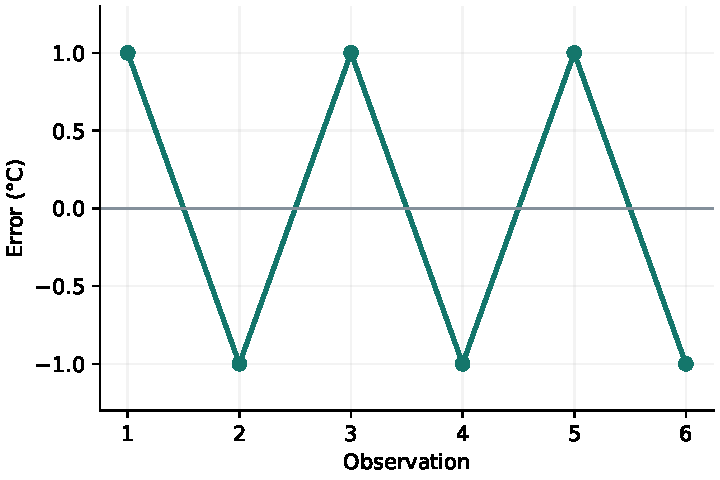
\includegraphics[width=\linewidth]{baseline.pdf}
  \caption{Baseline}\label{fig:baseline}
 \end{subfigure}\hfill
 \begin{subfigure}{0.48\linewidth}
  \centering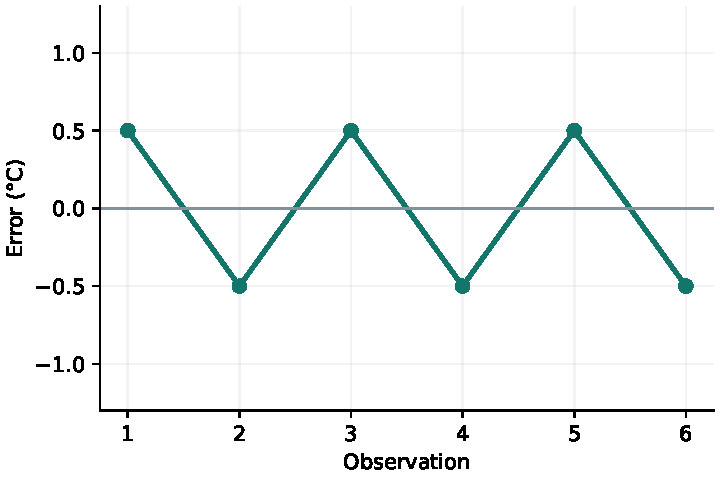
\includegraphics[width=\linewidth]{calibrated.pdf}
  \caption{Calibrated}\label{fig:calibrated}
 \end{subfigure}
 \caption{两种方法的误差对比（教学合成数据）。}\label{fig:comparison}
\end{figure}

\end{document}
